\documentclass[12pt, letterpaper, titlepage, hidelinks]{article}

% Packages
\usepackage[letterpaper, margin=1in]{geometry}
\usepackage[utf8]{inputenc}
\usepackage{fancyhdr}
\usepackage{setspace}
\usepackage{chemfig}
\usepackage{amssymb}
\usepackage{amsmath}
\usepackage{multirow}
\usepackage{array}
\usepackage{graphicx}
\usepackage{tabularx}
\usepackage{booktabs}
\usepackage{hyperref}
\usepackage{scrextend}
\usepackage{verbatim}
\usepackage[english]{babel}
\usepackage{blindtext}
\usepackage{capt-of}
\usepackage{float}
\usepackage{caption}
\usepackage{apacite}
\usepackage{mathrsfs}
\usepackage{siunitx}
\usepackage{booktabs}
\usepackage [autostyle, english = american]{csquotes}
\MakeOuterQuote{"}

\graphicspath{ {Images/} }


\floatstyle{plain}
\newfloat{calc}{thp}{lop}
\floatname{calc}{Calculation}

\newenvironment{nospaceflalign*}
{\setlength{\abovedisplayskip}{0px}\setlength{\belowdisplayskip}{0px}%
	\csname flalign*\endcsname}
{\csname endflalign*\endcsname\ignorespacesafterend}

% Title Page
\title{COMPENG 2SI4 Lab 1 \& 2 Report}
\author{Ashpan Raskar \\ raskara \\ 400185326}
\date{\today}



\begin{document}

\maketitle
\newpage
%\setcounter{secnumdepth}{0}
\section{Explanation of Methods}
	\subsection{Constructor (String Parameter)}
	\label{section:constructor-string}
		Method begins by performing a regular expression operation by checking if the entire string only contains the digits 0 to 9, or checks if the first character in the string is a "-" and then checks if the rest are digits only containing 0 to 9. If this condition is not met, an Illegal Argument Exception error is thrown to ensure an incorrect value cannot proceed.\\
		After that, it is determined where in the string the number actually begins, to prevent leading zeros and negatives to be accounted for to start. If there is a negative sign, then the "isNegative" class field is set to true.\\
		Then to store the number, an array is used, by checking the length of the string, setting that as the size of the array. The string is iterated and each value is added to that array.
	\subsection{Constructor (Integer Parameter)}
	\label{section:constructor-rng}
		Method begins by creating a new random object. Then the integer parameter (n) is checked if it is not 1 or greater. If it is not, then an Illegal Argument Exception error is thrown to ensure an incorrect value cannot proceed.\\
		Once we know the value is valid, an array of size "n" is created. Then it is populated with random digits varying from 0-9, except for the most significant digit, which is populated with a random digit from 1-9, to ensure no leading zeros exist.
	\subsection{Addition}
	\label{section:add}
		Let $a$ be the absolute of first number, $b$ be the absolute of second number\\
		The addition method begins by checking 2 cases where addition will not actually be used, the cases with only of the 2 numbers is negative.\\ Ex: $-a + b$ OR $a + (-b)$\\
		In these cases, instead of addition, subtraction will be used. To accomplish this, the subtract function is called with the appropriate values passed into the parameters.
		\subsubsection{Case 1: First Number Negative, Second Number Positive}
			If $|a| > b$, the result is equal is $b - |a|$ with the field value "isNegative" = true.\\
			If $|a| \leq b$, the result is equal to $b - |a|$ with the field value "isNegative" = false (to signify a positive answer)
		\subsubsection{Case 2: First Number Positive, Second Number Negative}
			If $a$ is positive and $b$ is negative\\
			If $|b| > a$, the result is equal is $a - |b|$ with the field value "isNegative" = true.\\
			If $|b| \leq a$, the result is equal to $a - |b|$ with the field value "isNegative" = false (to signify a positive answer)
		\subsubsection{Case 3: Both Positive or Both Negative}
			After considering those two cases, and not belonging to either case (aka, both positive or both negative), it moves to the next stage. We create a copy of the 2 HugeIntegers to one called "longer" and another called "shorter", this will be used to store the 2 HugeIntegers based on their lengths and easily keep track which one is longer and shorter.\\
			A StringBuilder object is used to easily append the values to it without implicitly knowing its length.\\
			The method will iterate from the least significant digit (LSD) to the most significant digit (MSD) to add them together. The modulus of the sum of each digit and carry by 10 is taken as the value that is appended to the string; and the integer division of the sum of each digit and carry by 10 is stored in a carry variable to add to the next significant digits.\\
			This will repeat until the shorter number runs out of digits, once this occurs the sum, modulus, and integer division, will be done with only the next digit on the longer number and the carry variable.\\
			Finally the negative states are checked, and if both number have a negative, a "-" is inserted into the beginning of the string and finally returned as a HugeInteger object, passing in the string as the constructor parameter.
	\subsection{Subtraction}
	\label{section:subtract}
		Let $a$ be the absolute of first number, $b$ be the absolute of second number.\\
		For the cases where both are not positive, they will use the addition function as specified in \nameref{section:add}.
		\subsubsection{Case 1: Both Negative}
			Result is $-a + |b|$
		\subsubsection{Case 2: First Negative, Second Positive}
			Result is $-(|a| + b)$
		\subsubsection{Case 3: First Positive, Second Negative}
			Result is $a + |b|$
		\subsubsection{Case 4: Both Positive}
			If $a \geq b$ isNegative field is false, otherwise isNegative is true.\\
			Create bigger and smaller HugeInteger objects to easily keep track of longer and shorter HugeIntegers.\\
			Iterate from the LSD to MSD for both values, if the borrow variable is true, reduce the current digit in the bigger object by 1.\\
			Then check if the bigger object digit minus smaller object digit is $\geq 0$, if so, set borrow to true, and then increase current bigger object digit by 10 (this borrows a number from the next digit) and set borrow to true.\\
			If that statement is false, then set borrow to false.\\
			After that append the subtraction of smaller from bigger to the string. Once the smaller object runs out of digits, operations will only be done with the bigger object. If borrow is set to true, reduce the digit by one and then set it to false. After that the rest of the digits will just be brought down.\\
			If the negative variable is true, insert a "-" at the beginning of the string.\\
			Finally  a HugeInteger object is returned, passing in the string as the constructor parameter.
	\subsection{Multiplication}
	\label{section:multiply}
		This method starts by determining if the output will be negative or positive by checking if only 1 of the 2 numbers is negative. If true, it sets "negative" to true, otherwise to leaves "negative" as false.\\
		Then the bigger and smaller objects are created to keep track of the longer and shorter HugeIntegers.\\
		Create a sum HugeInteger which will eventually contain the answer of the multiplication, initialize this with a value of 0.\\
		Iterate through the bigger object from LSD to MSD. Everytime a digit from "bigger" is iterated through, create a new "answer" StringBuilder to contain the answer of that row of multiplication. Also create a counter which determines which digit of "bigger" is currently being dealt with so that 0's can be appended to the answer.\\
		Create another for loop iterating through the LSD to MSD of the smaller object.\\
		Insert the current "bigger" digit times the "smaller" digit plus the carry all taken of the modulus of 10.\\
		Then the carry is equal to current "bigger" digit times the "smaller" digit plus the carry all taken of the integer division of 10.\\
		If there is a carry left over after iterating through all digits in "smaller", then add that to the string in the MSD position. Then add "counter" number of digits in the LSD position to account for the current "bigger" digit.\\
		Then create a HugeInteger object with the string passed into the constructor.\\
		After than add this new HugeInteger to the "sum" HugeInteger. This will repeat for all digits in the 2 HugeIntegers.
		Finally, set the negative if required, and then return "sum".
	\subsection{Compare To}
	\label{section:compare}
		\subsubsection{Case 1: First Number Negative, Second Number Positive}
			Return -1 to specify second number larger.
		\subsubsection{Case 2: First Number Positive, Second Number Negative}
			Return 1 to specify first number larger.
		\subsubsection{Case 3: First Number Negative, Second Number Negative}
			If the length of the first one is larger than the second one then return -1 to specify second number is larger.\\
			If the length of the second one is larger than the first one then return 1 to specify first number is larger.\\
			Otherwise, iterate through the number from MSD to LSD and if the first number has a larger digit than the second number, return -1. If the second number has a larger digit than the first number, return 1.\\
			If all the digits are the same, return 0.\\

		\subsubsection{Case 4: First Number Positive, Second Number Positive}
			If the length of the first one is larger than the second one then return 1 to specify first number is larger.\\
			If the length of the second one is larger than the first one then return -1 to specify second number is larger.\\
			Otherwise, iterate through the number from MSD to LSD and if the first number has a larger digit than the second number, return 1. If the second number has a larger digit than the first number, return -1.\\
			If all the digits are the same, return 0.\\
\section{HugeInteger Memory Computation}
	Given a HugeInteger of $n$ digits, the below outlines a calculation of the memory required to store this value.\\
	The class contains 2 field values:\\
	1. An array of $n$ integers\\
	2: A boolean containing the negative state of the integer\\\\
	Size of Integer $= 4$ bytes\\
	Size of n elements Array $= n\cdot$ size of elements in array\\
	Size of Boolean $= 9$ bytes\\
	Total size of HugeInteger object $= 4\cdot n + 9$ bytes.\\\\
	Example: Size of HugeInteger with 3419 digits $= 4\cdot 3419 + 9 = 13685$ bytes $\approx 13.36$ kilobtyes.
\section{Extra Memory Computations for Methods}
	\subsection{Addition}
		During the addition method, an extra 2 Huge Integer objects are created.\\
\indent		$2\cdot (4n+9) = 8n+18$ bytes.\\
		2 integers are also created.\\
\indent		$2\cdot 4 = 8$ bytes.\\
		1 String with a max length of $n+2$ is created.\\
\indent		$2\cdot (n+2) + 4 = 2n+8$ bytes\\
		Adding all of these together gives us:\\
\indent		$8n+18 + 8 + 2n + 8 = 10n + 34$ bytes
	\subsection{Subtraction}
		During the subtraction method, an extra 2 Huge Integer objects are created.\\
\indent		$2\cdot (4n+9) = 8n+18$ bytes.\\
		2 booleans are used to store the negative state and borrow variable.\\
\indent		$2\cdot9 = 18$ bytes.\\
		2 integers are also created.\\
\indent		$2\cdot 4 = 8$ bytes.\\
		1 String with a max length of $n+1$ is created.\\
\indent		$2\cdot (n+1) + 4 = 2n+6$ bytes\\
		Adding all of these together gives us:\\
\indent		$8n+18 + 18 + 8 + 2n+6 = 10n + 50$ bytes

	\subsection{Multiplication}
		During the multiplication method, an extra 2 Huge Integer objects are created.\\
\indent		$2\cdot (4n+9) = 8n+18$ bytes.\\
		1 boolean is used to store the negative state.\\
\indent		$2\cdot9 = 18$ bytes.\\
		2 integers are also created to store the counter and carry variables.\\
\indent		$2\cdot 4 = 8$ bytes.\\
		1 String with a max length of $2n-1$ is created.\\
\indent		$2\cdot (2n-1) + 4 = 4n+2$ bytes\\
		Adding all of these together gives us:\\
\indent		$8n+18 + 18 + 8 + 4n+2 = 12n + 46$ bytes
	
	\subsection{Compare To}
		During compare to, no extra memory is required to perform this method.\\
\indent		$0$ bytes.

\section{Big Theta ($\Theta$) Run Time}
\subsection{Addition}
The add method iterates through the maximum length of the largest HugeInteger, aka size $n$, this means that the big theta run time is $\Theta(n)$
\subsection{Subtraction}
The subtract method operates similar to the add method, it iterates through the maximum length of the largest HugeInteger, aka size $n$, this means that the big theta run time is $\Theta(n)$
\subsection{Multiplication}
The multiplication iterates through both the length of the larger HugeInteger and smaller HugeInteger, this means the total iterations is $n\times m$, this means that at max the big theta run time is $\Theta(n^2)$
\subsection{Compare To}
The compare to function checks through a variety of if statements, without using any loops. This shows that the $\Theta(1)$.
\newpage

\section{Run Time Complexity}
Average running time was measuring using the built in function System.currentTimeMillis(). The average running time was determined by calculating run time for many computations and then the total time was divided by the given computations. This was then repeated for different digit sizes of the Big and Huge Integers.\\
\begin{table}[H]
	\centering
	\begin{tabular}{lllllll}
		\toprule
		Method     & MAXNUMINTS & MAXRUN    & n     & Huge (ms)     & Big  (ms)     & Scaled Theoretical\\ \midrule
		Addition   & 100        & 2000000   & 10    & 4.10E-08 & 1.58E-09 & 10\\
		Addition   & 100        & 500000    & 100   & 8.89E-07 & 9.58E-09 & 100\\
		Addition   & 100        & 10000     & 1000  & 7.78E-04 & 2.91E-06 & 1000\\
		Addition   & 100        & 500       & 10000 & 0.429564 & 3.32E-04 & 10000\\ \midrule
		Subtract   & 100        & 2000000   & 10    & 4.25E-08 & 1.72E-09 & 10\\
		Subtract   & 100        & 500000    & 100   & 6.87E-07 & 8.00E-09 & 100\\
		Subtract   & 100        & 10000     & 1000  & 5.65E-04 & 2.07E-06 & 1000\\
		Subtract   & 100        & 500       & 10000 & 0.428576 & 4.12E-04 & 10000\\ \midrule
		Multiply   & 100        & 50000     & 10    & 6.00E-05 & 1.43E-07 & 100\\
		Multiply   & 100        & 200       & 100   & 0.717825 & 3.50E-04 & 10000\\
		Multiply   & 100        & 2         & 1000  & 11406    & 3.5      & 1000000\\ \midrule
		Compare To & 100        & 300000000 & 10    & 2.54E-13 & 7.52E-13 & 1\\
		Compare To & 100        & 300000000 & 100   & 2.19E-13 & 6.98E-13 & 1\\
		Compare To & 100        & 300000000 & 1000  & 7.65E-13 & 6.01E-13 & 1\\
		Compare To & 100        & 300000000 & 10000 & 2.45E-13 & 9.06E-13 & 1\\ \bottomrule
	\end{tabular}
\end{table}
\begin{figure}[H]
	\centering
	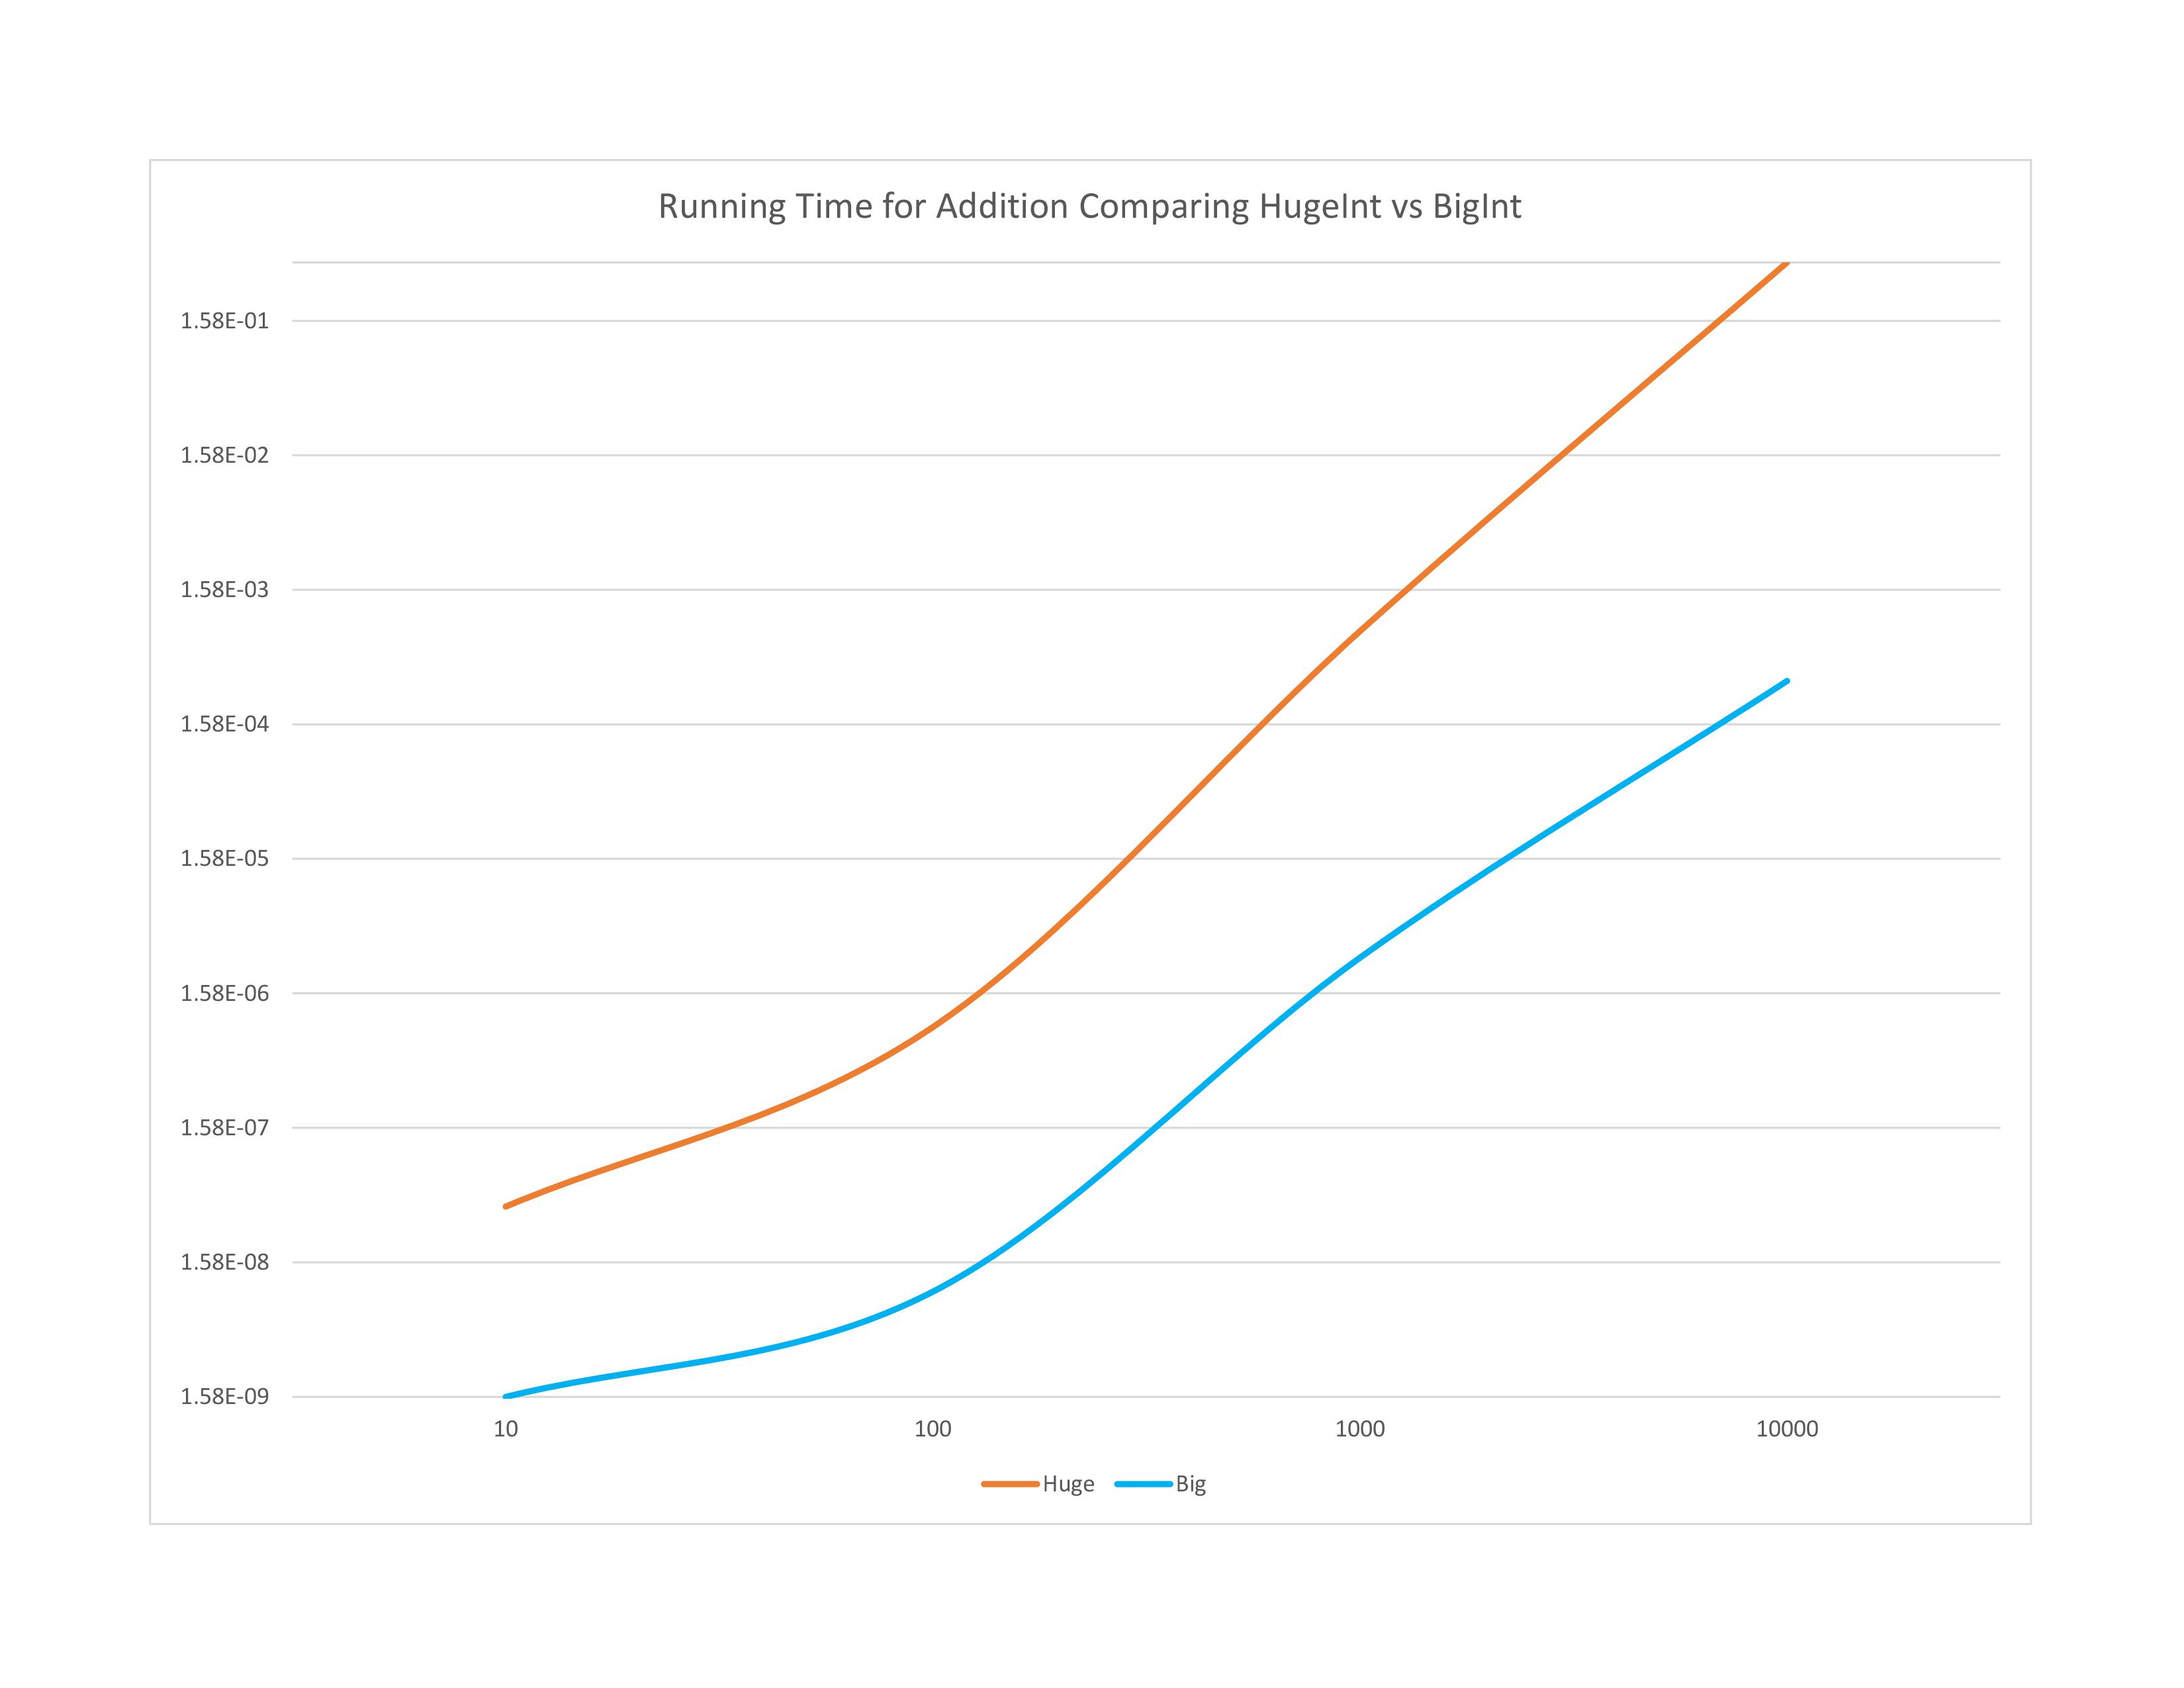
\includegraphics[width=0.49\textwidth]{add}
	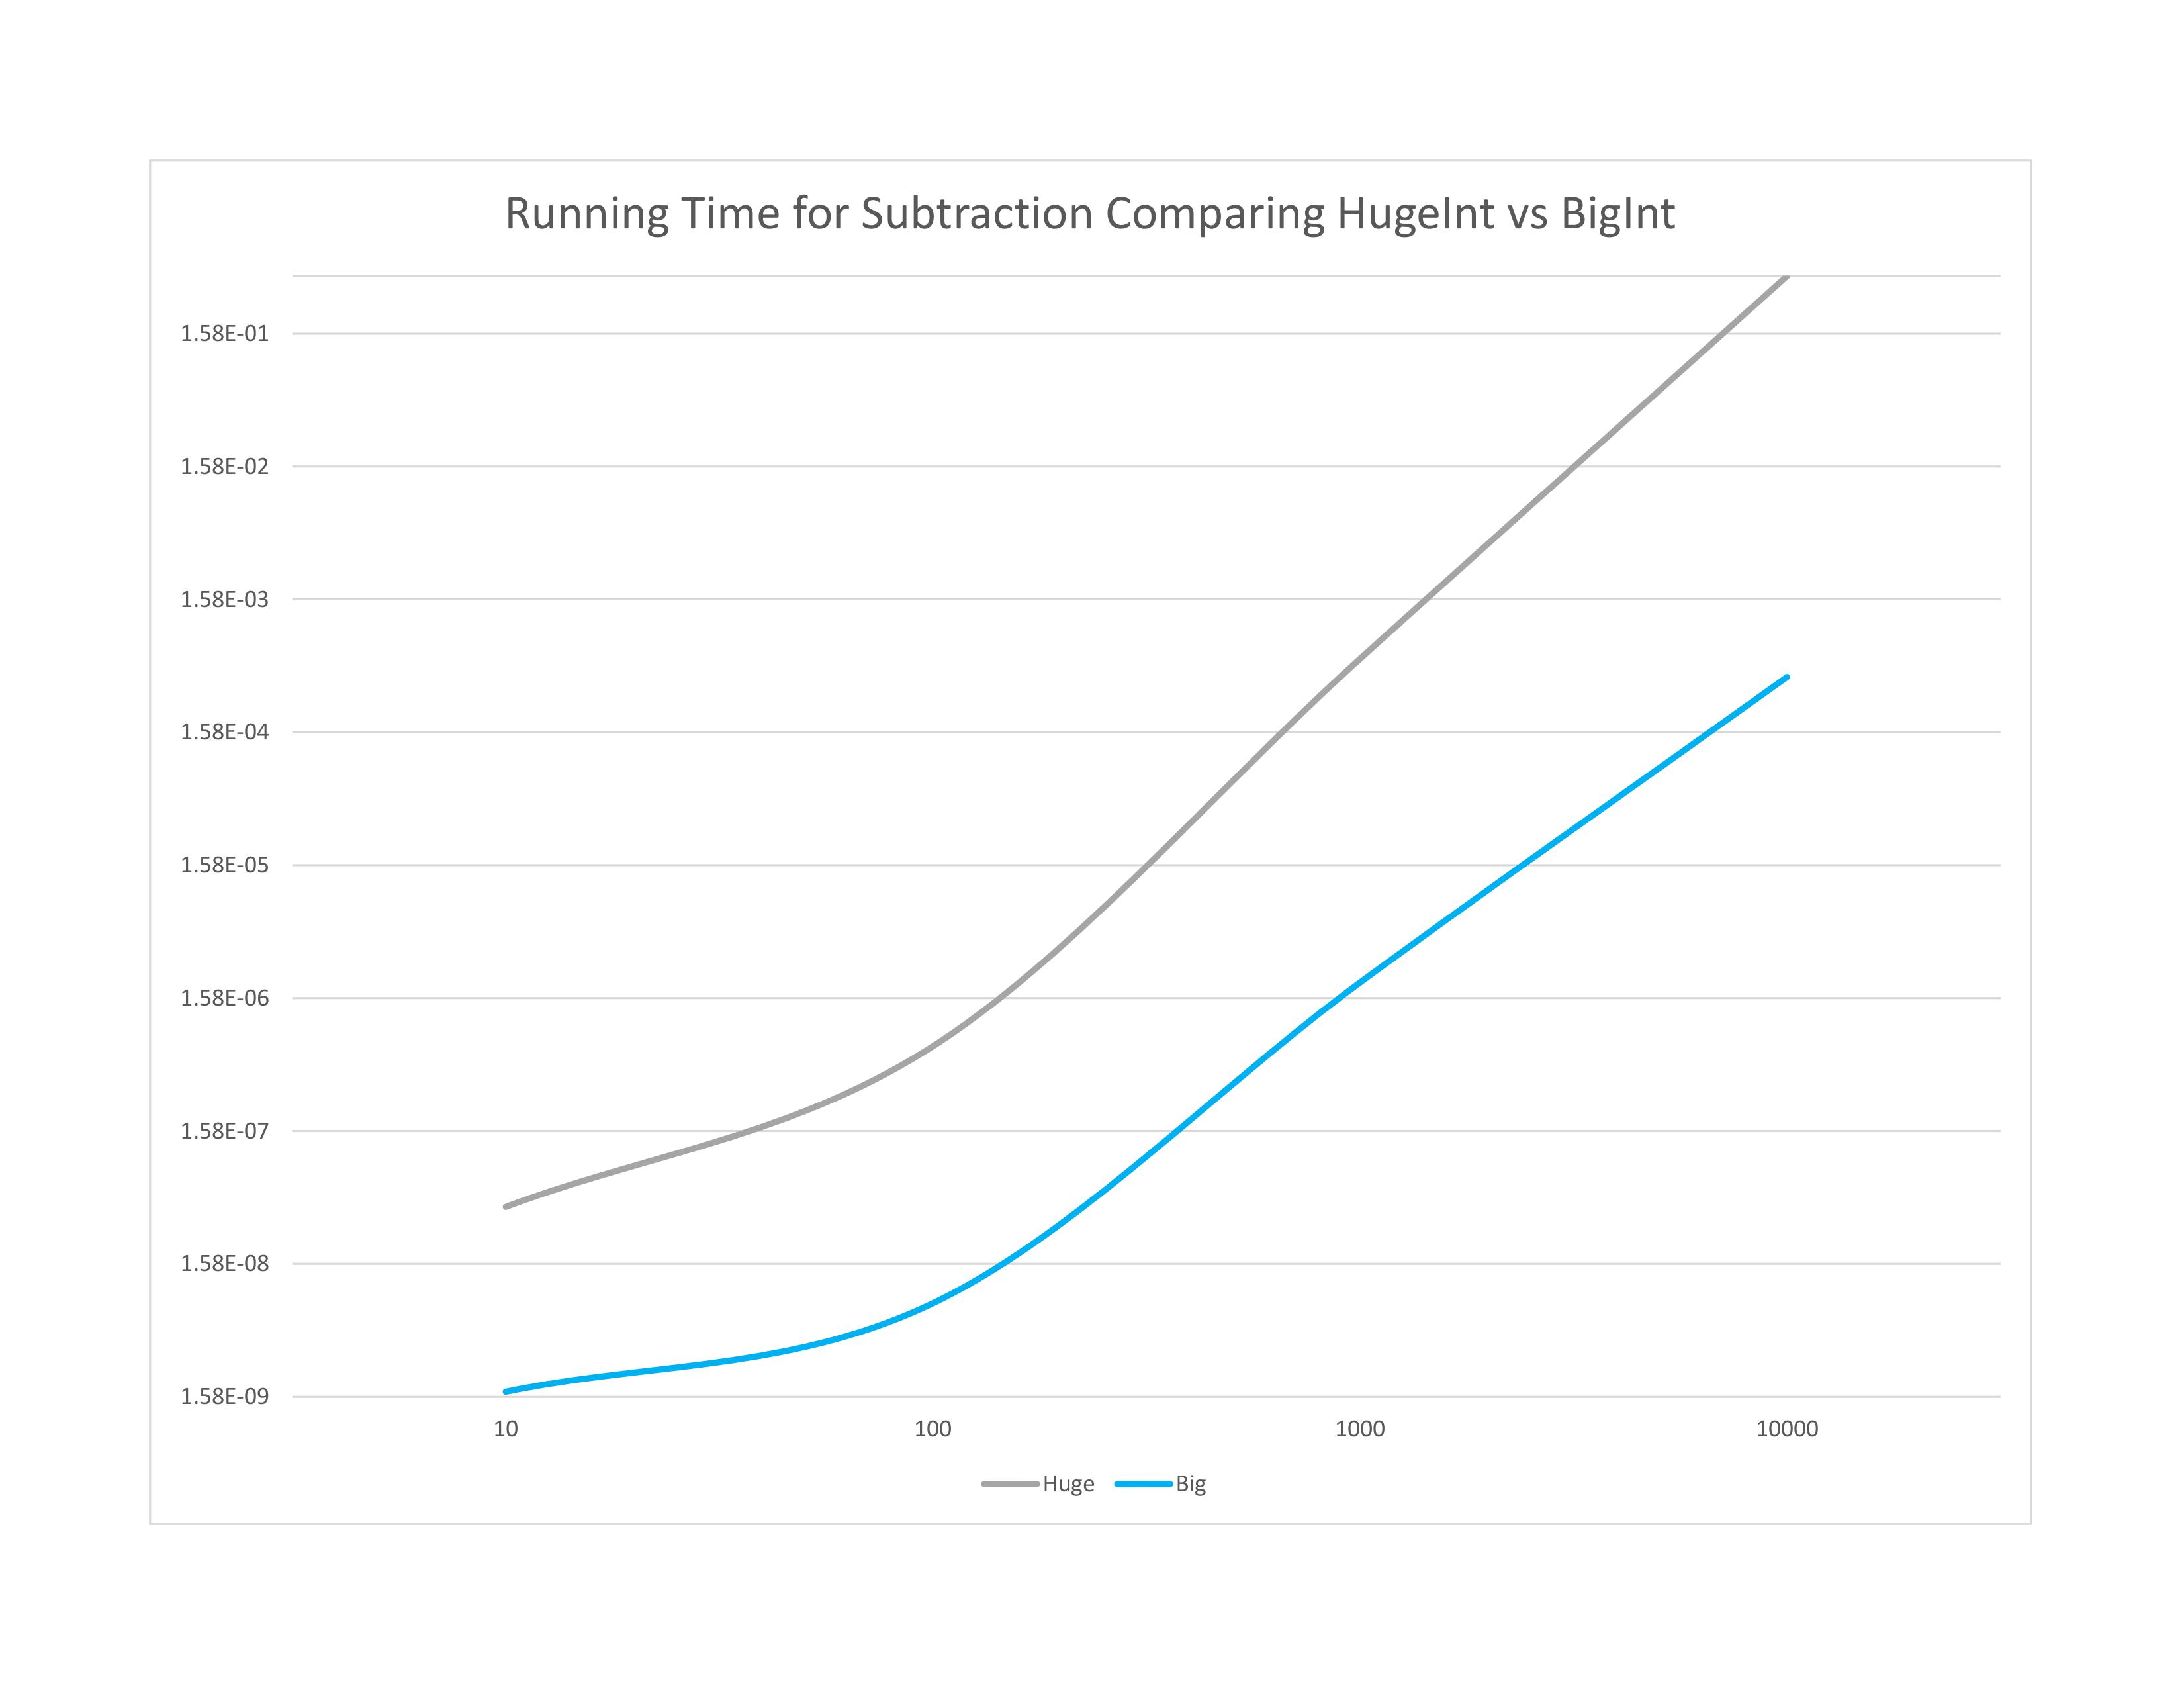
\includegraphics[width=0.49\textwidth]{sub}
\end{figure}
\begin{figure}[H]
	\centering
	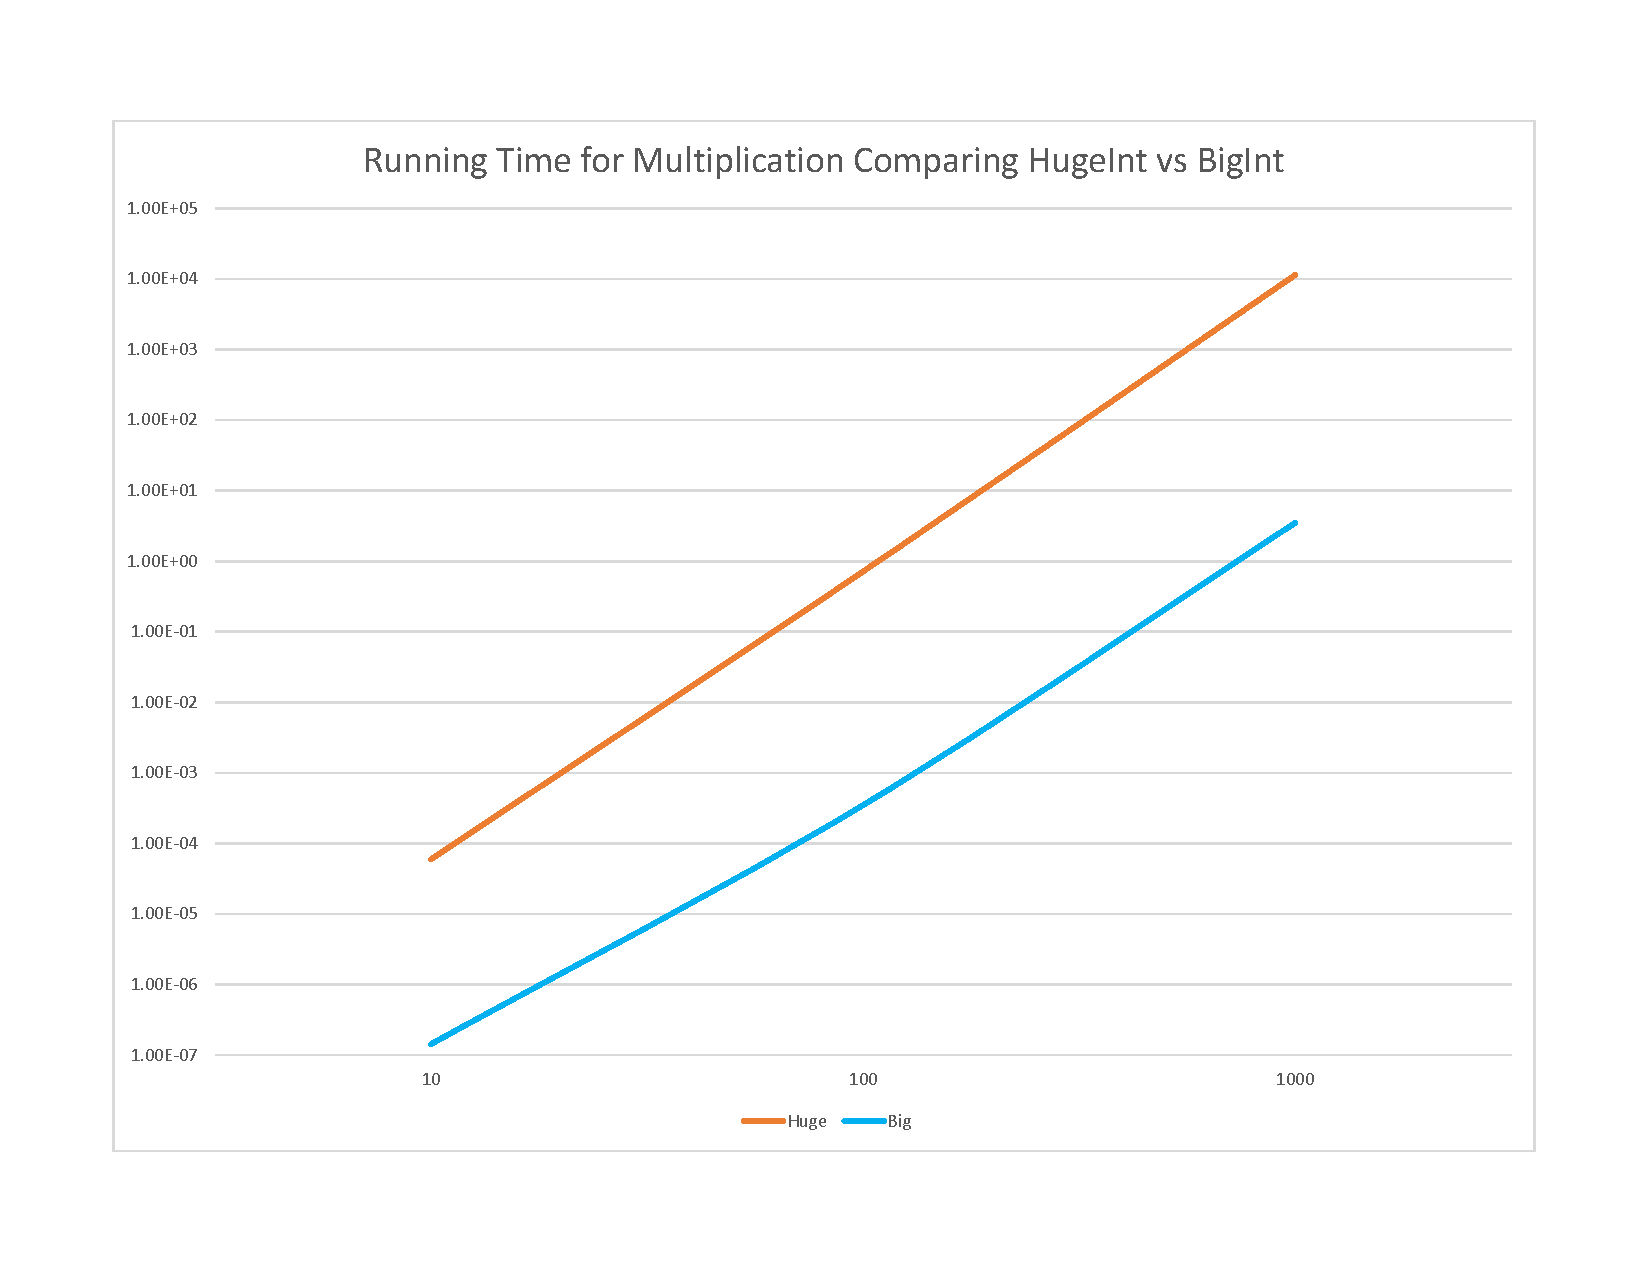
\includegraphics[width=0.49\textwidth]{mult}
	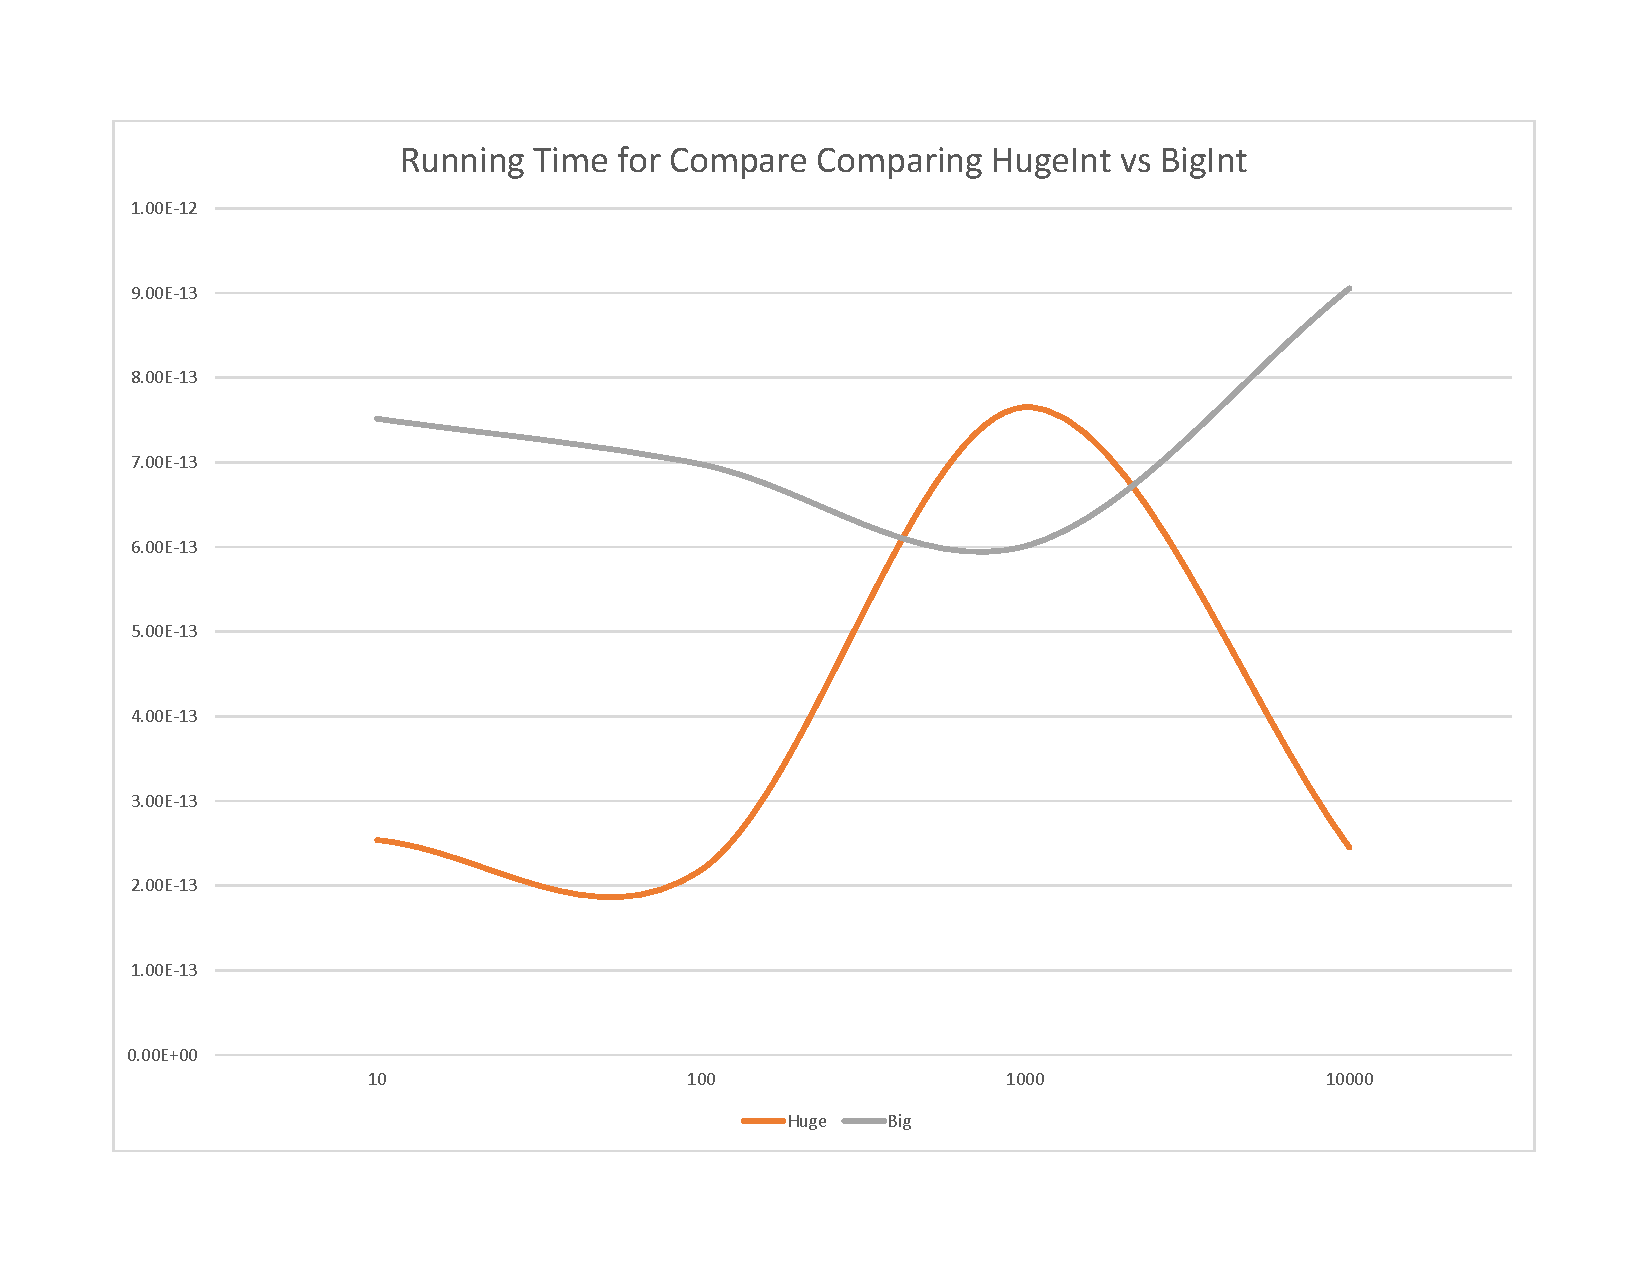
\includegraphics[width=0.49\textwidth]{comp}	
\end{figure}
\section{Discussion}
	My theoretical calculations compared to the measured run time is quite accurate. For the addition and subtraction they grew linearly. Whereas the multiplication function had a faster growth rate of $n^2$. The compare function has a theoretical calculation of $\Theta(1)$, and this showed to be true as all the run times had a magnitude of $a\cdot 10^-13$ which says that the run time is a constant regardless of $n$.\\
	After testing each function with each test case (eg: Invalid parameters, negative plus positive, negative plus negative, positive plus negative, positive plus positive, negative minus positive, negative minus negative, etc), no bugs were apparent and it seemed to work exactly as expected.\\
	The runtime of my code versus the BigInteger built in Java class, was slower than theirs. In the graphs it can be seen that my program is slower by a factor of $10^3$ for addition, $10^2$ for subtraction, and $10^4$ for multiplication. But for the compare to the run times are very similar.\\
	To improve my program, I believe I would have to reconstruct my algorithm to operate without any strings, as this would use less memory as well as reduce to runtime of my method to become closer to the BigInteger class. This would require me to operate in only HugeInteger objects instead of strings.
	
\end{document}          
